\section{Implementation}
\label{sec:implementation}

In this section the implementation of the chatroom is examined in depth. Firstly, the extension for the client side and then for the server side are described respectively. Lastly the chat system is explained in greater detail, since it encapsulates our work for Milestone 5.

\subsection{Client Side Implementation}
\label{sec:Implementation_clintside}

\begin{figure}[h]
	\centering
	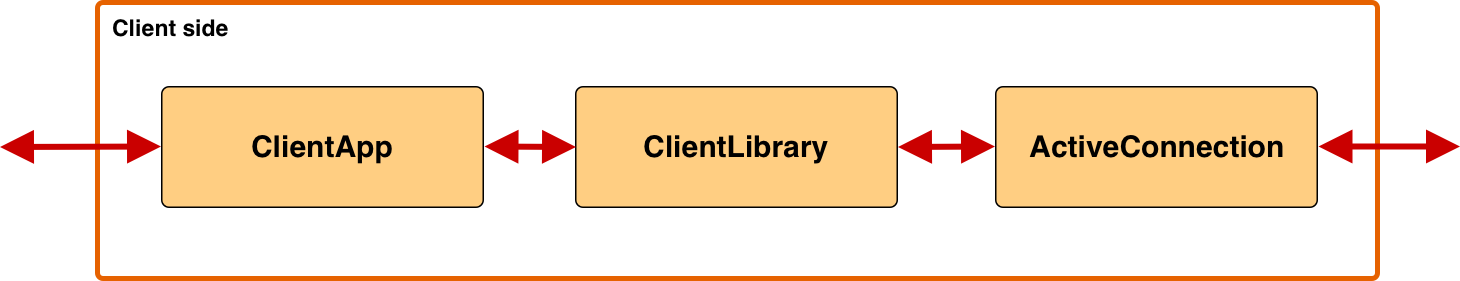
\includegraphics[width=\linewidth]{figures/client_arch.png}
	\caption{Client side architecture}
	\label{fig:client_arch}
\end{figure}
The client side consists of the three following main components as seen in figure \ref{fig:client_arch}:
\begin{enumerate} 
  \item \textit{ClientApp} represents the client interface which allows input through the console. From there the client is able to issue commands to: connect to and disconnect from the system, interact with the key-value store and chat. The input is then checked and parsed before getting sent to the ClientLibrary. The result of the user command is displayed on the console through the ClientApp.
  \item \textit{ClientLibrary} serves as a bridge between the client and the server.
  \item \textit{ActiveConnection} abstracts the TCP socket connection to the server which allows the client to connect to the server socket and exchange data without worrying about the underlying structure.
\end{enumerate}
 
\subsection{Server Side Implementation}
\label{sec:implementation_serverside}

Each server owns a list containing the active chatrooms that it is responsible for. In order for a client to join one of those chatrooms is that it would first need to connect to that server, similar to the way storing key-value pair functions. The decision, to make chatrooms accessible only from one server has both its advantages and disadvantages. For one, it reduces the complexity of the system because otherwise servers would need a way to exchange updates regarding the active chatrooms and chat users whenever a user joins or leaves.

A problem with our implementation is that if the chatIDs are not equally distributed across all servers, which may occur due to the unpredictable nature of the hashing function, a single server could then be in charge of most chatrooms. This would cause that a server to be overloaded with requests and would lead to greater response times and, in the worst-case scenario, would result in a bottleneck for the whole system. In order to combat this issue, we limit the number of chatrooms belonging to one server to 15 and the number of users in a single chatroom to 30. This means a server is responsible for up to 450 chat users. These limits could also be easily changed depending on the intended use case of the system.

The biggest advantage of our decision is that it heavily reduces network traffic. Since all chatroom users are connected to the same server, that server can easily forward messages between them. Otherwise additional socket connections would have been required which would have both increased the load on the network and the overall complexity of the system.

Our idea for the chatting functionality was for it to be as lightweight as possible with clients entering and leaving chatrooms regularly.

\subsection{Chat System}
\label{sec:implementation_chatsystem}
The chat system consists of three main components as namely:
\begin{enumerate}
	\item \textit{ChatManager}, who is in charge of providing all chat functionalities to the client, including connecting to a chatroom and sending messages.
	\item \textit{ChatRoom}, which is identified by a chatID. A Chatroom object contains a map of all connected users and their sockets, in order to be able to forward messages.
	\item \textit{ChatBot}, which is responsible to execute PUT and GET commands during a chat session. The chatbot acts exactly like a client, meaning it first has to connect to the responsible server and then send its request.
	
By utilizing a chatbot, chat requests containing a key-value operation are slowed down, since only one "client" is performing those operations. However, if each chat user is tasked with executing the commands himself instead, then whenever a key is located at a server different from the server responsible for the chatroom, the client would need to reconnect twice. Not only that, but also all chat messages sent while the user was disconnected would either get lost or will be displayed after the user has reconnected, which would make the user temporarily unavailable. As mentioned in section \ref{sec:background_cap}, our system focuses on being available. 	

\end{enumerate}